\documentclass[preprint,12pt,aps,pra,showkeys,amsmath,amssymb,superscriptaddress,floatfix]{revtex4-2}
\usepackage[T1]{fontenc}
\usepackage[utf8]{inputenc}
\usepackage{amsmath,amssymb,amsthm,mathtools,mathrsfs}
\usepackage{microtype,booktabs,enumitem}
\usepackage{xcolor,tikz,etoolbox}
\usepackage[skins,breakable]{tcolorbox}
\usepackage{needspace}
% Keep diagram geometry independent of REVTeX preprint body spacing.
\AtBeginEnvironment{tikzpicture}{\linespread{1}\selectfont}
\usetikzlibrary{arrows.meta,positioning,calc,fit,decorations.pathreplacing}
\usepackage{graphicx}
\usepackage{hyperref}

\definecolor{MMBlue}{RGB}{0,82,155}
\definecolor{MMOrange}{RGB}{200,80,0}
\tikzset{
 mmnode/.style={draw=MMBlue,rounded corners=2pt,fill=MMBlue!4,align=left,execute at begin node={\raggedright},text width=5cm,font=\fontsize{10}{12}\selectfont,inner sep=6pt},
 mmimport/.style={mmnode,draw=black!65,fill=black!4},
 mmcandidate/.style={mmnode,draw=MMOrange,dashed,fill=MMOrange!5},
 mmrejected/.style={mmnode,draw=black,densely dotted,fill=black!8},
 mmproof/.style={->,thick,MMBlue},
 mmflow/.style={->,semithick,black!70},
 mmrepair/.style={->,dashed,thick,MMOrange},
 mmcandidatearrow/.style={->,dashed,semithick,MMOrange},
 mmnote/.style={font=\scriptsize,fill=white,inner sep=2pt,align=center}}

\usepackage[section]{placeins}
\setlength{\emergencystretch}{3em}
\setlist{itemsep=3pt,topsep=4pt}
\newtheorem{theorem}{Theorem}[section]
\newtheorem{proposition}[theorem]{Proposition}
\newtheorem{lemma}[theorem]{Lemma}
\newtheorem{corollary}[theorem]{Corollary}
\theoremstyle{definition}
\newtheorem{definition}[theorem]{Definition}
\newtheorem{example}[theorem]{Example}
\theoremstyle{remark}
\newtheorem{remark}[theorem]{Remark}
% Avoid isolated statement headings and single-line paragraph fragments.
\BeforeBeginEnvironment{theorem}{\Needspace{6\baselineskip}}
\BeforeBeginEnvironment{definition}{\Needspace{5\baselineskip}}
\BeforeBeginEnvironment{proposition}{\Needspace{5\baselineskip}}
\BeforeBeginEnvironment{lemma}{\Needspace{5\baselineskip}}
\BeforeBeginEnvironment{corollary}{\Needspace{5\baselineskip}}
\clubpenalty=5000
\widowpenalty=5000
\newcommand{\R}{\mathbb R}\newcommand{\Z}{\mathbb Z}\newcommand{\N}{\mathbb N}
\newcommand{\Pa}{\operatorname{Pa}}\newcommand{\Desc}{\operatorname{Desc}}
\newcommand{\cl}{\operatorname{cl}}\newcommand{\cost}{\operatorname{cost}}
\newcommand{\status}{\operatorname{status}}
% Faculty cards: a visual rail groups the five faculties within one agent.
% The rail has no arrowhead and does not represent a proof dependency.
\newcommand{\mmfacultybadge}[1]{%
 \node[circle,draw=MMBlue,line width=1pt,fill=white,
 minimum size=7mm,inner sep=0pt,font=\sffamily\small\bfseries,text=MMBlue]
 at ([xshift=15pt,yshift=-15pt]frame.north west) {#1};}
\newcommand{\mmfacultyrail}{%
 \draw[MMBlue!80,line width=1pt]
 ([xshift=15pt,yshift=2pt]frame.north west)--
 ([xshift=15pt,yshift=-2pt]frame.south west);}
\newtcolorbox{mmfacultybox}[2]{enhanced,breakable,
 colback=MMBlue!4,colframe=MMBlue!4,boxrule=0pt,arc=3pt,
 left=39pt,right=9pt,top=4pt,bottom=4pt,
 before skip=2pt,after skip=2pt,
 fontupper=\small\linespread{1.1}\selectfont,
 overlay unbroken={\mmfacultyrail\mmfacultybadge{#1}},
 overlay first={\mmfacultyrail\mmfacultybadge{#1}},
 overlay middle={\mmfacultyrail},overlay last={\mmfacultyrail}}
\newcommand{\mmfaculty}[3]{%
 \begin{mmfacultybox}{#1}{#2}
 {\sffamily\bfseries\color{MMBlue}#2}\par\smallskip #3
 \end{mmfacultybox}}
\newcommand{\agent}[9]{%
 \Needspace{8\baselineskip}
 \subsubsection{#1}
 \noindent\textbf{Object.} #2\par
 \noindent\textbf{Role.} #3\par\smallskip
 \mmfaculty{E}{Ego}{#4}
 \mmfaculty{M}{Memory}{#5}
 \mmfaculty{I}{Intellect}{#6}
 \mmfaculty{S}{Sense}{#7}
 \mmfaculty{A}{Action}{#8}
 \smallskip\noindent #9\par}

\usepackage{longtable,array,calc}
\providecommand{\tightlist}{\setlength{\itemsep}{2pt}\setlength{\parskip}{0pt}}
\makeatletter
\def\frontmatter@abstract@produce{\par\addvspace{\frontmatter@preabstractspace}%
\begingroup\prep@absbox\unvbox\absbox\post@absbox\endgroup
\addvspace{\frontmatter@postabstractspace}}
\makeatother
\newcommand{\field}[2]{\par\smallskip\noindent\textbf{#1.} #2\par}
\setlength{\emergencystretch}{5em}
\AtBeginEnvironment{verbatim}{\small\linespread{1.0}\selectfont}


\hypersetup{colorlinks=true,linkcolor=MMBlue,urlcolor=MMBlue,pdfauthor={Dibakar Sigdel}}

\begin{document}

\title{Poisson Summation Formula\\[4pt]\large An End-to-End Meta-Math Walkthrough}

\author{Dibakar Sigdel}

\affiliation{Mindverse Computing LLC, Lynnwood, WA 98087, USA}

\date{October 2026}

\begin{abstract}

A complete authored walkthrough of poisson summation formula, with
explicit mathematical contracts, local verification gates, and reusable
exports. The report presents the target theorem, declared imports, a
dependency graph, five-faculty node contracts, a continuous proof, a
worked example, and a hypothesis-repair audit. It is an authored
mathematical exposition, not a deployed-agent transcript or a formal
proof-assistant certificate.

\end{abstract}\maketitle\linespread{1.12}\selectfont

\noindent\textbf{HA-05 / Harmonic Analysis / Report v1}

\section{Target and import contract}

\begin{theorem}

For \(f\in\mathcal S(\mathbb R)\) with HA-04's Fourier convention, prove
\(\sum_{n\in\mathbb Z}f(n)=\sum_{k\in\mathbb Z}\widehat f(k)\).

\end{theorem}

\subsection{Foundations and permitted imports}

Use Schwartz rapid-decay bounds for f and its derivatives. Import
uniqueness of Fourier coefficients for continuous periodic functions
from HA-03, scaled to period1; if a continuous function has all
coefficients zero, \(L^{2}\) density makes it zero everywhere. Only
absolutely convergent integrals and sums are interchanged.

\clearpage\section{Node interaction workflow}

\begin{center}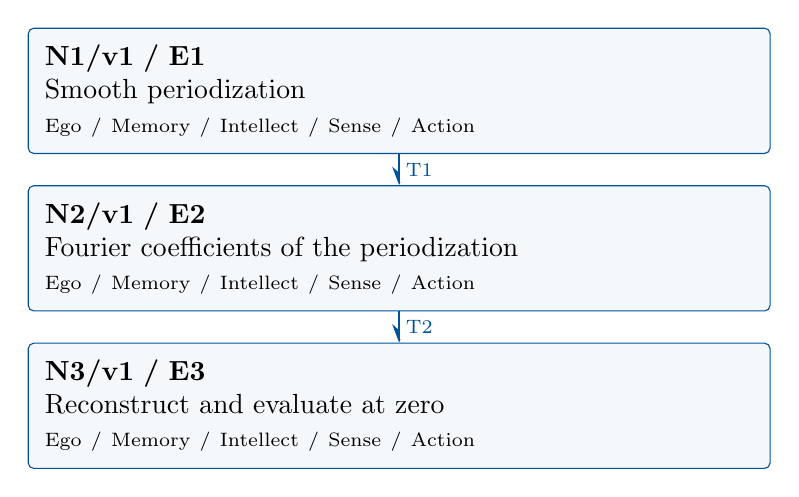
\begin{tikzpicture}[>=Stealth,x=1cm,y=1cm]

\node[mmnode,text width=9cm,minimum height=1.25cm] (N1) at (0,0.0) {\textbf{N1/v1 / E1}\\Smooth periodization\\{\scriptsize Ego / Memory / Intellect / Sense / Action}};

\node[mmnode,text width=9cm,minimum height=1.25cm] (N2) at (0,-2.0) {\textbf{N2/v1 / E2}\\Fourier coefficients of the periodization\\{\scriptsize Ego / Memory / Intellect / Sense / Action}};

\node[mmnode,text width=9cm,minimum height=1.25cm] (N3) at (0,-4.0) {\textbf{N3/v1 / E3}\\Reconstruct and evaluate at zero\\{\scriptsize Ego / Memory / Intellect / Sense / Action}};

\draw[mmproof] (N1.south) -- node[mmnote,right] {T1} (N2.north);

\draw[mmproof] (N2.south) -- node[mmnote,right] {T2} (N3.north);

\end{tikzpicture}\end{center}

Each box is one mathematical agent containing all five faculties. Blue
arrows carry the versioned exports listed below. The layout gives a
reading order; only drawn arrows assert dependencies. Diagnostic repair
is separate from the proof DAG.

\subsection{Versioned evidence-transfer ledger}

\begingroup\small\linespread{1.05}\selectfont

\Needspace{5\baselineskip}\field{T1: N1/E1/v1 to N2}{A smooth periodic function P with absolutely convergent periodization.}

\field{Receiving activity}{N2: Fourier coefficients of the periodization}

\field{Compatibility}{Use the same mathematical objects and hypotheses as the source export.
Receiving contract: Uniform summability on{[}0,1{]}; prior exports E1/v1}

\Needspace{5\baselineskip}\field{T2: N2/E2/v1 to N3}{The kth coefficient of P is \(\widehat f(k)\).}

\field{Receiving activity}{N3: Reconstruct and evaluate at zero}

\field{Compatibility}{Use the same mathematical objects and hypotheses as the source export.
Receiving contract: Smooth P and identified coefficients; prior exports
E2/v1}

\endgroup

\clearpage\section{Agent roles and five-faculty activities}\begingroup\small\linespread{1.05}\selectfont\setlist{itemsep=1pt,topsep=2pt}

\subsection{N1/v1: Smooth periodization}

\field{Object and role}{Use rapid decay uniformly on a fundamental interval.}

\field{Inputs}{\(f\in S(R)\); foundational imports stated in §1}

\mmfaculty{E}{Ego}{Own E1/v1: A smooth periodic function P with absolutely convergent
periodization.}

\mmfaculty{M}{Memory}{Retain \(f\in S(R)\); foundational imports stated in §1; keep their
assumptions and versions attached.}

\mmfaculty{I}{Intellect}{Use rapid decay uniformly on a fundamental interval.}

\mmfaculty{S}{Sense}{Decay estimates must be uniform in x, not merely pointwise.}

\mmfaculty{A}{Action}{Carry out the numbered deductions and publish E1/v1 together with its
hypotheses and proof location.}

\smallskip\noindent\textbf{Numbered mathematical activities}

\begin{enumerate}[label=N1.\arabic*,leftmargin=3.4em]

\item For \(x\in [0,1]\) and each derivative orderr,
\(|f^{(r)}(x+n)|\le C_r(1+|n|)^{(-2)}\) after enlarging the constant for
finitely many n.

\item Hence \(P(x)=\sum _n\) \(f(x+n)\) and every derivative series converge
uniformly absolutely.

\item Termwise differentiation shows P is smooth; shifting the integer index
shows P is 1-periodic.

\end{enumerate}

\field{Export E1/v1}{A smooth periodic function P with absolutely convergent periodization.}

\field{Acceptance gate}{Decay estimates must be uniform in x, not merely pointwise. Publish only
after checking every displayed deduction.}

\field{Targeted repair}{If the check fails, revise N1: Decay estimates must be uniform in x, not
merely pointwise. Recheck dependent nodes N2, N3.}

\clearpage

\subsection{N2/v1: Fourier coefficients of the periodization}

\field{Object and role}{Unfold the integral into all translated intervals.}

\field{Inputs}{Uniform summability on{[}0,1{]}; prior exports E1/v1}

\mmfaculty{E}{Ego}{Own E2/v1: The kth coefficient of P is \(\widehat f(k)\).}

\mmfaculty{M}{Memory}{Retain Uniform summability on{[}0,1{]}; prior exports E1/v1; keep their
assumptions and versions attached.}

\mmfaculty{I}{Intellect}{Unfold the integral into all translated intervals.}

\mmfaculty{S}{Sense}{The integer k is crucial for the phase cancellation.}

\mmfaculty{A}{Action}{Carry out the numbered deductions and publish E2/v1 together with its
hypotheses and proof location.}

\smallskip\noindent\textbf{Numbered mathematical activities}

\begin{enumerate}[label=N2.\arabic*,leftmargin=3.4em]

\item For \(k\in Z\), its Fourier coefficient is
\(\int _{0}^{1}P(x)e^{(-2\pi ikx)}dx=\sum _n\int _{0}^{1}f(x+n)e^{(-2\pi ikx)}dx\).

\item Substitute \(u=x+n\).

\item Since \(e^{(2\pi ikn)}=1\), the sum of integrals over{[}n,n+1{]} equals
\(\int _R\) \(f(u)e^{(-2\pi iku)}du=\widehat f(k)\).

\item All rearrangements follow from absolute integrability.

\end{enumerate}

\field{Export E2/v1}{The kth coefficient of P is \(\widehat f(k)\).}

\field{Acceptance gate}{The integer k is crucial for the phase cancellation. Publish only after
checking every displayed deduction.}

\field{Targeted repair}{If the check fails, revise N2: The integer k is crucial for the phase
cancellation. Recheck dependent nodes N3.}

\clearpage

\subsection{N3/v1: Reconstruct and evaluate at zero}

\field{Object and role}{Prove absolute Fourier convergence before point evaluation.}

\field{Inputs}{Smooth P and identified coefficients; prior exports E2/v1}

\mmfaculty{E}{Ego}{Own E3/v1: Poisson summation for Schwartz functions with the stated
Fourier convention.}

\mmfaculty{M}{Memory}{Retain Smooth P and identified coefficients; prior exports E2/v1; keep
their assumptions and versions attached.}

\mmfaculty{I}{Intellect}{Prove absolute Fourier convergence before point evaluation.}

\mmfaculty{S}{Sense}{An \(L^{2}\) identity alone would not license evaluation at a chosen
point.}

\mmfaculty{A}{Action}{Carry out the numbered deductions and publish E3/v1 together with its
hypotheses and proof location.}

\smallskip\noindent\textbf{Numbered mathematical activities}

\begin{enumerate}[label=N3.\arabic*,leftmargin=3.4em]

\item Integrating by parts twice in the coefficient formula for periodic P,
with matching endpoint derivatives, gives
\(|\widehat f(k)|\le \Vert P''\Vert _{1}/(4\pi ^{2}k^{2})\) for
\(k\ne 0\).

\item Thus \(Q(x)=\sum _k\) \(\widehat f(k)e^{(2\pi ikx)}\) converges
uniformly absolutely and is continuous.

\item Its coefficients equal those of P by termwise integration.

\item Fourier uniqueness makes \(P=Q\).

\item \(Atx=0\) this gives \(\sum _n\) \(f(n)=P(0)=Q(0)=\sum _k\)
\(\widehat f(k)\).

\item Both numerical series are absolutely convergent.

\end{enumerate}

\field{Export E3/v1}{Poisson summation for Schwartz functions with the stated Fourier
convention.}

\field{Acceptance gate}{An \(L^{2}\) identity alone would not license evaluation at a chosen
point. Publish only after checking every displayed deduction.}

\field{Targeted repair}{If the check fails, revise N3: An \(L^{2}\) identity alone would not
license evaluation at a chosen point. Withhold this terminal result
until its gate passes.}

\endgroup\clearpage\section{Continuous mathematical proof}\label{sec:proof}

Read these steps in order as one proof; the diagram is optional.
Numbered activities identify the specific constructions and deductions
owned by each node.

\subsection{§4.N1 --- Smooth
periodization}\label{n1-smooth-periodization}

\begin{enumerate}
\def\labelenumi{\arabic{enumi}.}
\item
  For \(x\in [0,1]\) and each derivative orderr,
  \(|f^{(r)}(x+n)|\le C_r(1+|n|)^{(-2)}\) after enlarging the constant
  for finitely many n.
\item
  Hence \(P(x)=\sum _n\) \(f(x+n)\) and every derivative series converge
  uniformly absolutely.
\item
  Termwise differentiation shows P is smooth; shifting the integer index
  shows P is 1-periodic.
\end{enumerate}

\subsection{§4.N2 --- Fourier coefficients of the
periodization}\label{n2-fourier-coefficients-of-the-periodization}

\begin{enumerate}
\def\labelenumi{\arabic{enumi}.}
\item
  For \(k\in Z\), its Fourier coefficient is
  \(\int _{0}^{1}P(x)e^{(-2\pi ikx)}dx=\sum _n\int _{0}^{1}f(x+n)e^{(-2\pi ikx)}dx\).
\item
  Substitute \(u=x+n\).
\item
  Since \(e^{(2\pi ikn)}=1\), the sum of integrals over{[}n,n+1{]}
  equals \(\int _R\) \(f(u)e^{(-2\pi iku)}du=\widehat f(k)\).
\item
  All rearrangements follow from absolute integrability.
\end{enumerate}

\subsection{§4.N3 --- Reconstruct and evaluate at
zero}\label{n3-reconstruct-and-evaluate-at-zero}

\begin{enumerate}
\def\labelenumi{\arabic{enumi}.}
\item
  Integrating by parts twice in the coefficient formula for periodic P,
  with matching endpoint derivatives, gives
  \(|\widehat f(k)|\le \Vert P''\Vert _{1}/(4\pi ^{2}k^{2})\) for
  \(k\ne 0\).
\item
  Thus \(Q(x)=\sum _k\) \(\widehat f(k)e^{(2\pi ikx)}\) converges
  uniformly absolutely and is continuous.
\item
  Its coefficients equal those of P by termwise integration.
\item
  Fourier uniqueness makes \(P=Q\).
\item
  \(Atx=0\) this gives \(\sum _n\) \(f(n)=P(0)=Q(0)=\sum _k\)
  \(\widehat f(k)\).
\item
  Both numerical series are absolutely convergent.
\end{enumerate}

\hfill$\square$

\section{Worked orchestration}

For \(f(x)=e^(-\pi t\) \(x^{2}\)), \(t>0\), the Gaussian transform is
\(t^{(-1/2)}e^{(-\pi \xi ^{2}/t)}\). Thus \(\sum _n\) \(e^(-\pi t\)
\(n^{2})=t^{(-1/2)}\sum _k\) \(e^{(-\pi k^{2}/t)}\). At \(t=1\) the two
series agree termwise; at other t the formula relates different Gaussian
scales.

\subsection{Boundary and hypothesis audit}

Changing a function only at integers leaves its Lebesgue Fourier
transform unchanged but can change the left-hand sampled sum. This shows
why arbitraryL \(^{1}\) equivalence classes cannot satisfy a
point-sampling formula without additional regularity. Sense retains the
Schwartz scope.

\section{Illustrative failure and repair}

The following is an authored diagnostic scenario. Changed assumptions
define a new contract; they do not retroactively prove the original
statement.

\subsection{Failure and correction}
This is an authored teaching trace, not a recorded agent run.

\begin{enumerate}
\def\labelenumi{\arabic{enumi}.}
\tightlist
\item
  \textbf{Ego \(\to\) Memory:} register the §1 theorem, imports, and
  requested exports before beginning the proof.
\item
  \textbf{Intellect \(\to\) Action:} choose the bridges in §3 and carry
  out the numbered activities in §4; transmit only established E-exports
  along the §2 DAG.
\item
  \textbf{Sense \(\to\) responsible node:} test the specific
  boundary/failure in §5 and the node's individual audit. A failing
  candidate is withheld; downstream nodes may not use it.
\item
  \textbf{Memory + Intellect:} identify whether the error is an omitted
  condition, an invalid inference, or an attempted extension beyond the
  theorem. Restore the exact contract or explicitly state a different
  one.
\item
  \textbf{Action:} redo the affected mathematical activity using the
  repaired condition or inference. Recheck consuming nodes, rather than
  feeding their conclusions back as premises.
\item
  \textbf{Ego:} publish only the supported export with its assumptions
  and proof location. A hypothetical revised export is v2; the written
  proof here is the v1 exposition, not a claim that this repair was
  executed.
\end{enumerate}

\subsection{Hypothesis boundary}
Changing a function only at integers leaves its Lebesgue Fourier
transform unchanged but can change the left-hand sampled sum. This shows
why arbitraryL \(^{1}\) equivalence classes cannot satisfy a
point-sampling formula without additional regularity. Sense retains the
Schwartz scope.

\subsection{Version and recheck}
Treat any changed assumption as a new contract. Recheck the revised
export and all of its descendants. A backward diagnostic never
establishes an earlier theorem. This is an authored teaching trace, not
an execution log.

\par\medskip\begingroup\small\linespread{1.0}\selectfont\noindent\textbf{Provenance.} This authored proof is complete relative to its declared imports. Reuse
each export with its assumptions, proof, and version. The original
Markdown remains available for comparison.
\par\endgroup

\end{document}
